\documentclass[a4]{article}

\usepackage[left=3cm,right=3cm,top=2cm,bottom=2cm]{geometry} 

\usepackage[utf8]{inputenc}   % otra alternativa para los caracteres acentuados y la "ñ"
\usepackage[           spanish % para poder usar el español
                      ,es-tabla % para los captions de las tablas
                       ]{babel}   
\decimalpoint %para usar el punto decimal en vez de coma para los números con decimales

\usepackage[T1]{fontenc}
\usepackage{lmodern}

\usepackage{parskip}
\usepackage{xcolor}

\usepackage{caption}
\usepackage{hyperref}
\usepackage{enumerate} % paquete para poder personalizar fácilmente la apariencia de las listas enumerativas
\usepackage{listings}
\usepackage{xcolor}
\usepackage{amsmath}
\definecolor{codegreen}{rgb}{0,0.6,0}
\definecolor{codegray}{rgb}{0.2,0.2,0.2}
\definecolor{codepurple}{rgb}{0.58,0,0.82}
\definecolor{backcolour}{rgb}{0.95,0.95,0.92}

\lstdefinestyle{mystyle}{
	backgroundcolor=\color{backcolour},   
	commentstyle=\color{codegray},
	keywordstyle=\color{codegreen},
	numberstyle=\tiny\color{blue},
	stringstyle=\color{red},
	basicstyle=\ttfamily\normalsize,
	breakatwhitespace=false,         
	breaklines=true,                 
	captionpos=b,                    
	keepspaces=true,                 
	numbers=left,                    
	numbersep=5pt,                  
	showspaces=false,                
	showstringspaces=false,
	showtabs=false,                  
	tabsize=2
}

\lstset{style=mystyle}
\usepackage{graphicx} % figuras
\usepackage{subfigure} % subfiguras

\usepackage{amsfonts}
\usepackage{amsmath}

\definecolor{gris}{RGB}{220,220,220}
	
\usepackage{float} % para controlar la situación de los entornos flotantes

\restylefloat{figure}
\restylefloat{table} 

%%Sobre el código
\usepackage{xparse}
\NewDocumentCommand{\codeword}{v}{%
	\texttt{\textcolor{blue}{#1}}%
}



\newcommand{\HRule}{\rule{\linewidth}{0.5mm}}

\author{Pilar Navarro Ramírez y Alejandro Miguel Palencia Blanco}
\date{\vspace{-5mm}}

\title{\huge APRENDIZAJE AUTOMÁTICO: Proyecto final\\Devanagari Handwritten Character Dataset \HRule\vspace{-4mm}}

\usepackage[ruled]{algorithm2e}

\begin{document}
\maketitle
\tableofcontents

\newpage

\section{Definición del problema}

Dada una imagen de un carácter de Devanagari manuscrito, se busca  identificar cuál es dicho carácter. Así, se parte de un conjunto de 92000 imágenes con caracteres manuscritos por muchos individuos diferentes, de manera que hay gran variedad en la forma en que se escribe cada carácter. Cada imagen está en escala de grises con el carácter sobre un fondo negro (píxeles con valor 0) y es de $32\times32$ píxeles. Se dispone además de una etiqueta asociada a cada imagen, que indica el carácter representado en la misma. En total hay 46 clases a las que un carácter puede pertenecer, 36 letras y 10 dígitos. 

Nos encontramos, por lo tanto, ante un problema de aprendizaje supervisado, pues disponemos de una muestra etiquetada para el aprendizaje. En concreto se trata de un problema de clasificación multietiqueta, ya que hay 46 clases diferentes en las que queremos clasificar los carateres. 

Así pues, tenemos que el espacio de características $\mathcal{X}$ está formado por 92000 vectores con\\ $32\times32=1024$ valores entre 0 y 255 ($\mathcal{X}=[0,255]^{1024}$), correspondientes a los distintos valores de gris que puede tomar cada uno de los píxeles de la imagen. El conjunto de etiquetas $\mathcal{Y}$ consta de 46 clases diferentes, cada una para un carácter de Devanagari. La función objetivo $ f $ será la que, dado un vector de características del espacio $\mathcal{X}$ correspondiente a una imagen, determina la clase a la que pertenecerá el caracter representado en la imagen, es decir, al que corresponde el conjunto de píxeles de la imagen. 

\underline{Referencias:}

\href{https://archive.ics.uci.edu/ml/datasets/Devanagari+Handwritten+Character+Dataset}{https://archive.ics.uci.edu/ml/datasets/Devanagari+Handwritten+Character+Dataset}

\href{https://ieeexplore.ieee.org/stamp/stamp.jsp?tp=&arnumber=7400041}{Deep learning based large scale handwritten Devanagari character recognition}

\section{Conjuntos de entrenamiento y test}

Los datos que se nos proporcionan ya se encuentran separados en entrenamiento y test. Concretamente, en el conjunto de entrenamiento encontramos 1700 elementos por clase, lo que nos da un total de 78200 elementos (el 85\% del \textit{dataset}). Por otro lado, el conjunto de test dispone de 300 elementos por clase, dándonos un total de 13800 elementos (el 15\% del \textit{dataset}). Con esto se comprueba que las clases están totalmente balanceadas en ambos conjuntos.

Hemos decidido mantener estos conjuntos de entrenamiento y de test porque, además de estar en ellos las clases balanceadas, así podremos comparar nuestros resultados con otros estudios donde se utilizan exactamente los mismos conjuntos.

Para validar los modelos, haremos una partición del conjunto de entrenamiento en la que un 20\% del mismo será destinado para validación. Para ello, usamos la función \codeword{train_test_split} de \codeword{sklearn} con el parámetro \codeword{stratify} para mantener el balance entre las clases en ambos subconjuntos. Esto nos deja con 62560 elementos en el nuevo conjunto de entrenamiento y 15640 elementos en validación. Como podemos ver, nuestro conjunto de datos tiene un tamaño lo suficientemente grande como para llevar a cabo esta operación sin riesgo de que los conjuntos de entrenamiento y validación resultantes sean demasiado reducidos.



\section{Preprocesamiento}

Partimos de imágenes en escala de grises con una resolución de $32 \times 32$ píxeles. En ellas, el carácter se encuentra centrado en los 28x28 píxeles centrales, siendo el resto de píxeles el resultado de aplicar un \textit{padding} de tamaño 2 en los cuatro lados del carácter.

Al leer las imágenes, las etiquetas se codifican como números de 0 a 45. Estos valores pueden ser luego recodificados (por ejemplo, a vectores one-hot) según las necesidades de cada modelo.

\subsection{Cálculo del \textit{Bounding Box} y recortado de imágenes}

Lo primero que haremos será encontrar para cada carácter su \textit{Bounding Box} o caja englobante, para a continuación eliminar aquellos píxeles que se queden fuera de ella. Para ello, seguimos los siguientes pasos:

\begin{enumerate}
    \item Sobre una copia de la imagen, aplicamos la operación \textit{closing} mediante la función \codeword{morphologyEx} de la biblioteca \codeword{OpenCV}. Esta operación es útil para cerrar pequeños huecos o puntos negros que puedan encontrarse dentro del carácter.
    \item Luego, aplicamos un \textit{thresholding} con la función \codeword{threshold} de \codeword{OpenCV} para obtener una imagen binaria (en blanco y negro). Mediante esta operación, los píxeles que no superen un determinado umbral cambian a negro, mientras que el resto pasan a ser blancos. Hemos usado el método de Otsu para llevar a cabo el \textit{thresholding}.
    \item Por último, buscamos el rectángulo más pequeño que contenga a todos los píxeles blancos de la imagen binaria. Este rectángulo, que será el \textit{Bounding Box} del carácter, lo codificamos a partir de las coordenadas de su esquina superior izquierda, $(x,y)$, su anchura, $w$, y su altura, $h$.
\end{enumerate}

Una vez encontrado el \textit{Bounding Box}, lo usamos para recortar la imagen original en escala de grises. En la siguiente figura podemos ver una imagen del conjunto de datos a la que se le aplica este procedimiento.

\begin{figure}[H]
	\subfigure[Imagen original]{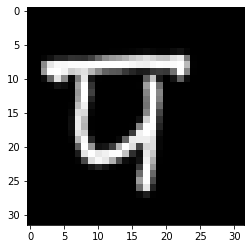
\includegraphics[width=51mm]{img/prep_example1.png}}
	\subfigure[Imagen después de \textit{closing}]{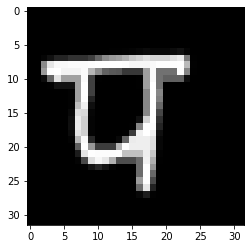
\includegraphics[width=51mm]{img/prep_example2.png}}
	\subfigure[Imagen después de \textit{thresholding} con su \textit{Bounding Box}]{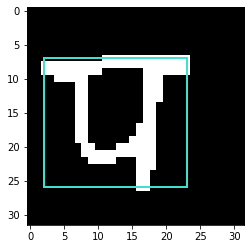
\includegraphics[width=51mm]{img/prep_example3.png}}
	\label{fig:prep_bounding_box}
\end{figure}

\underline{Referencias:}

\href{https://learnopencv.com/otsu-thresholding-with-opencv/}{https://learnopencv.com/otsu-thresholding-with-opencv/}    

\href{https://docs.opencv.org/master/d7/d4d/tutorial_py_thresholding.html}{https://docs.opencv.org/master/d7/d4d/tutorial\_py\_thresholding.html}

\href{https://docs.opencv.org/master/d9/d61/tutorial_py_morphological_ops.html}{https://docs.opencv.org/master/d9/d61/tutorial\_py\_morphological\_ops.html}

\subsection{Reescalado de imágenes}

Nada nos garantiza que los tamaños de las imágenes recortadas sean los mismos. Por tanto, es necesario aplicar algún tipo de reescalado para que todas ellas tengan el mismo tamaño. Lo ideal sería que este reescalado alterase lo menos posible las imágenes recortadas, así que hemos calculado la anchura y la altura medias de las imágenes recortadas para elegir de forma mucho más acertada las dimensiones de las imágenes reescaladas. 

La anchura y altura medias son $27.747$ y $26.895$, respectivamente, luego hemos decidido fijar a $27 \times 27$ las dimensiones del reescalado. Para llevarlo a cabo, usamos la función \codeword{resize} de \codeword{OpenCV} con interpolación bilineal. En la siguiente figura, podemos ver cómo queda la imagen anterior después de aplicarle el reescalado.

\begin{figure}[H]
    \centering
	\subfigure[Imagen después del reescalado]{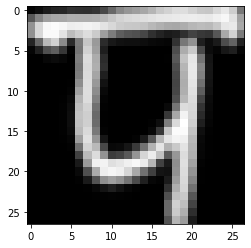
\includegraphics[width=51mm]{img/prep_example4.png}}
	\label{fig:prep_reescalado}
\end{figure}


\subsection{\textit{Downsampling}}

Con el objetivo de reducir la dimensionalidad de las imágenes, llevamos a cabo un \textit{downsampling} sobre todas ellas. Esto consiste en aplicar primero una convolución con un kernel gaussiano de dimensión $3 \times 3$ seguido de una reducción de tamaño en la que eliminamos las filas y las columnas pares. La convolución ha sido realizada mediante la función \codeword{GaussianBlur} de \codeword{OpenCV}. En la siguiente figura, podemos ver cómo queda la imagen anterior después de aplicarle el \textit{downsampling}.

\begin{figure}[H]
    \centering
	\subfigure[Imagen después del \textit{downsampling}]{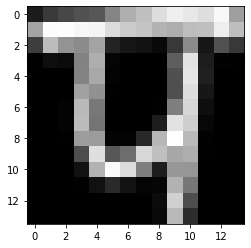
\includegraphics[width=51mm]{img/prep_example5.png}}
	\label{fig:prep_downsampling}
\end{figure}


Esta operación es arriesgada, pues estamos reduciendo la cantidad de información contenida en las imágenes. Para justificar que el \textit{downsampling} no perjudica al modelo, hemos ajustado cada uno de los modelos a partir de los datos preprocesados con esta transformación y sin ella (usando los mejores valores de los parámetros de los modelos obtenidos, que explicaremos más adelante). Luego, comparamos su rendimiento mediante la \textit{accuracy} que obtienen sobre el conjunto de validación. Los resultados se pueden ver en la siguiente tabla.

\begin{table}[H]
	\centering
	\begin{tabular}{|l|c|c|}
    \hline
    \multicolumn{1}{|c|}{\textbf{Modelos}} & \textbf{Con \textit{downsampling}} & \textbf{Sin \textit{downsampling}} \\ \hline
    Regresión Logística                    & 0.74815                & 0.75505                   \\ \hline
    Perceptrón Multicapa                   & 0.93939                & 0.93370                   \\ \hline
    Random Forest                          & 0.91905                & 0.91822                   \\ \hline
    SVM Gaussian-RBF                       & 0.96183                & 0.83990                   \\ \hline
    RBF-Network                            & 0.70511                & 0.76451                \\ \hline
    \end{tabular}
	\caption{\textit{Accuracy} obtenida por cada modelo en validación a partir de los datos preprocesados con y sin \textit{downsampling}}
	\label{table:downsampling}
\end{table}

Podemos comprobar que las \textit{accuracy} obtenidas en validación son muy similares, llegando incluso a ser significativamente inferior en SVM sin \codeword{downsampling}. Hemos decidido que \textit{downsampling} es una operación que en general favorece el aprendizaje, pues sintetiza la información más relevante reduciendo considerablemente la dimensionalidad de los datos. Esto, a su vez, nos permite aplicar validación cruzada en el ajuste de hiperparámetros sin que el coste computacional sea demasiado excesivo.

Las redes de funciones de base radial, sin embargo, son la excepción, pues presentan mejores resultados sobre los datos sin downsampling. Sin embargo, como veremos más adelante, este modelo requiere un tiempo de ejecución muy elevado y, si no reducimos la dimensionalidad, este tiempo de ejecución sería aún mayor. 


Antes de pasar a la última etapa del preprocesamiento, cambiamos la estructura matricial de las imágenes por una vectorial en la que las filas se concatenan una detrás de otra.

\underline{Referencias:}

\href{https://docs.opencv.org/master/d4/d86/group__imgproc__filter.html#gaf9bba239dfca11654cb7f50f889fc2ff}{https://docs.opencv.org/master/d4/d86/group\_\_imgproc\_\_filter.html\#gaf9bba239dfca11654cb7f50f889fc2ff}

\subsection{Eliminación de características constantes y normalización}

Las características constantes no aportan ninguna información relevante durante el ajuste del modelo, por ello, las eliminamos mediante la función \codeword{VarianceThreshold} de \codeword{sklearn}. Esta función, con sus valores por defecto, elimina aquellas características con varianza 0 (las que son constantes). Sin embargo, tras realizar esta operación, nos damos cuenta de que el conjunto de datos obtenido tras llevar a cabo las operaciones antes mencionadas no presenta características constantes, pues el número de características no disminuye tras la eliminación de las constantes.

Por último, aplicamos una normalización a las características restando su media y dividiendo por su desviación típica, esto es, hacemos que todas las características tengan media 0 y varianza 1. La normalización acelera la convergencia y, además, es necesaria para algunos de los modelos que vamos a usar de scikit-learn, como es el caso de SVM o MLP. Esto lo hacemos con la función \codeword{StandardScaler} de \codeword{sklearn}.

Con el preprocesamiento, hemos conseguido reducir la dimensionalidad de los datos de las\\ $32\times32=1024$ características originales, a simplemente 169, de manera que el aprendizaje será menos costoso. 

\section{Visualización de los datos}

Visualizamos los datos del conjunto de entrenamiento original y tras el preprocesamiento para tener una idea de la distribución de los mismos y del efecto del preprocesamiento. 
Para ello, necesitamos reducir el número de características a 2, para poder ver los datos en 2 dimensiones. Haremos uso de dos técnicas de reducción de la dimensionalidad: PCA (Principal Components Analysis) y t-SNE (t-Distributed Stochastic Neighbouring Entities). 

\textbf{PCA} es una técnica que usa la correlación entre las variables e intenta obtener a partir de ellas (mediante combinaciones lineales de las mismas) el mínimo número de variables posibles que expliquen una cierta variabilidad de los datos originales. Para ello, hace uso de los valores propios más grandes y vectores propios asociados a los mismos, de la matriz de correlaciones, pues estos últimos apuntan en la dirección de mayor variación en el conjunto de datos. Así, se transforma el espacio original de características en otro espacio diferente, intentando explicar la mayor proporción de la varianza de los datos posible. 

\textbf{T-SNE}, por su parte, se basa en la distribución de probabilidad de los vecinos alrededor de cada punto. En el espacio de caracterísitas multidimensional original ésta se modela como una distribución normal, mientras que en el nuevo espacio 2D se modela como una distribución t de Student. El objetivo de esta algoritmo es encontrar una proyección en el espacio 2D que minimice la diferencia entre estas dos distribuciones sobre todos los puntos. 

El parámetro principal que controla el ajuste es la perplejidad (\lstinline|perplexity|), que es el número de vecinos más cercanos considerados para hacer coincidir las distribuciones original y ajustada, en cada uno de los puntos. Con un valor bajo de la perplejidad nos centramos más en los puntos cercanos, en la escala local, mientras que un valor alto nos da una visión más general de los datos. Fijamos\\ \lstinline|perplexity=30|, un valor lo suficientemente alto como para tener una visión global de los datos. Valores entre 5 y 50 suelen producir los mejores resultados, como se indica en una de las referencias. 

Este algoritmo es costoso computacionalmente y es recomendable usar otra técnica de reducción de la dimensionalidad antes de aplicarla. Por ello, aplicaremos t-SNE partiendo de los datos obtenidos por PCA (\lstinline{init=x_pca}). 

T-SNE suele proporcionar mejores resultados para la visualización de los datos, de ahí que usemos ambas técnicas. 

Puesto que disponemos de una gran cantidad de datos en el conjunto de entrenamiento, para visualizarlos todos t-sne tardaría mucho tiempo y los gráficos obtenidos estarían demasidao cargados, de modo que a penas podríamos distinguir unos datos de otros. Por ello lo que hacemos es visualizar sólo la mitad del conjunto de entrenamiento. Para dividirlo hacemos uso de la función \lstinline{train_test_split}, quedándonos con un 50\% de los datos elegidos de forma aleatoria y estratificada, es decir, de manera que haya el mismo número de ejemplos en cada una de las clases. Así, se mantiene la distribución de los datos en las distintas clases. Como tenemos gran cantidad de datos, la mitad de ellos siguen siendo representativos de la distribución de los mismos.

Por otra parte, al haber 46 clases, no es posible visualizarlas todas en un mismo gráfico de manera que se distingan claramente los datos pertenecientes a cada clase. Por ello, para la representación, separamos las clases correspondientes a dígitos y  a letras, y este último grupo, a su vez, se divide en caracteres del 1 al 18 y caracteres del 19 al 36 .


Así, obtenemos las siguientes figuras:

\begin{figure}[H]
	\centering    
	\subfigure[Sin preprocesamiento]{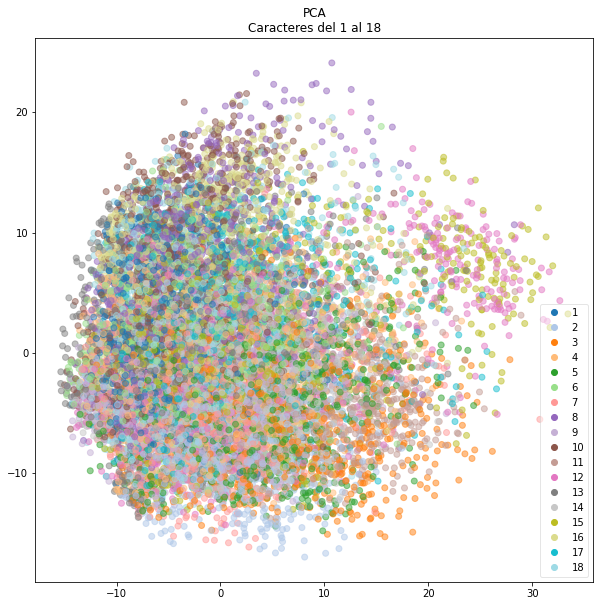
\includegraphics[width=77mm]{img/pca1_sin_prep.png}}
	\subfigure[Con preprocesamiento]{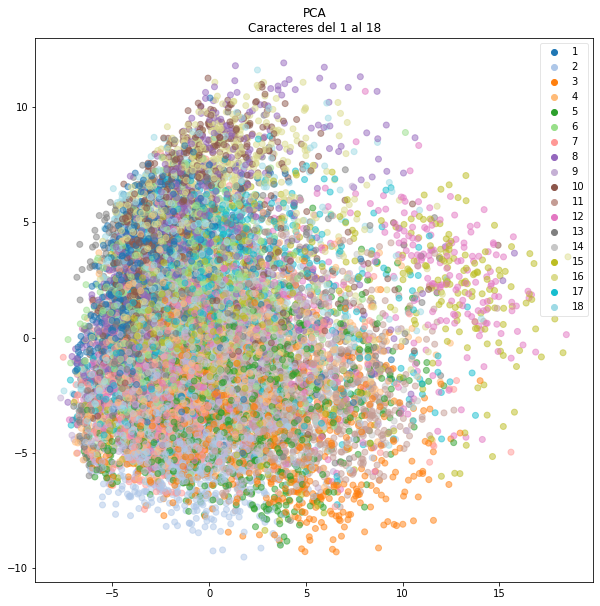
\includegraphics[width=77mm]{img/pca1_con_prep.png}}
	\subfigure[Sin preprocesamiento]{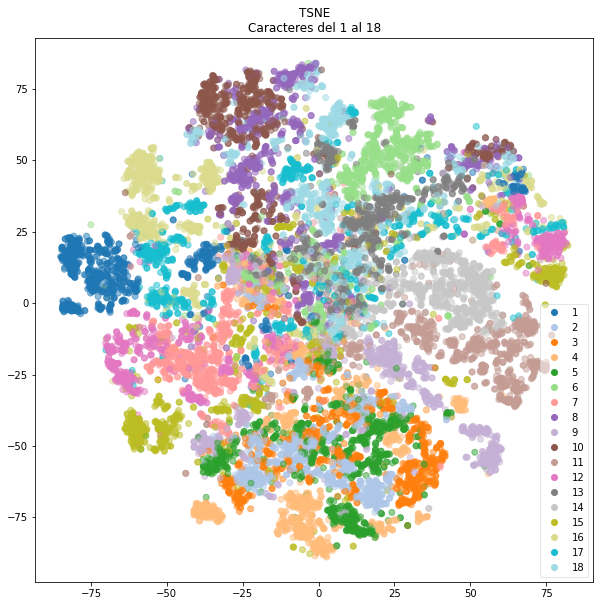
\includegraphics[width=77mm]{img/tsne1_sin_prep.png}}
	\subfigure[Con preprocesamiento]{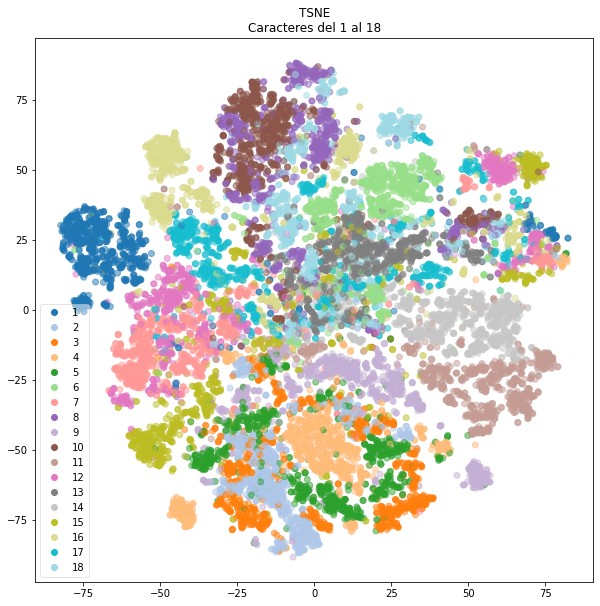
\includegraphics[width=77mm]{img/tsne1_con_prep.png}}
	\caption{Caracteres del 1 al 18}
	\label{fig:dimreduction1}
\end{figure}

\begin{figure}[H]
	\centering    
	\subfigure[Sin preprocesamiento]{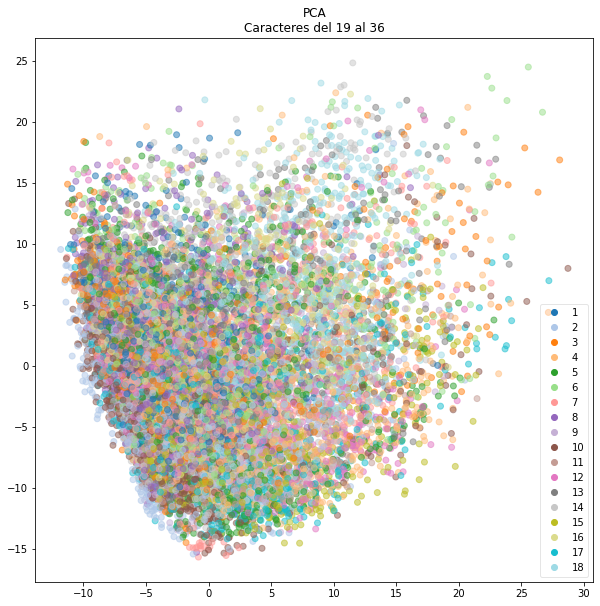
\includegraphics[width=77mm]{img/pca2_sin_prep.png}}
	\subfigure[Con preprocesamiento]{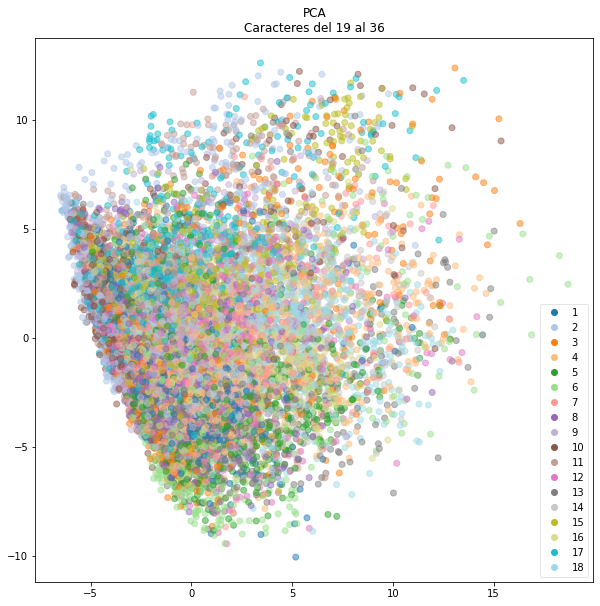
\includegraphics[width=77mm]{img/pca2_con_prep.png}}
	\subfigure[Sin preprocesamiento]{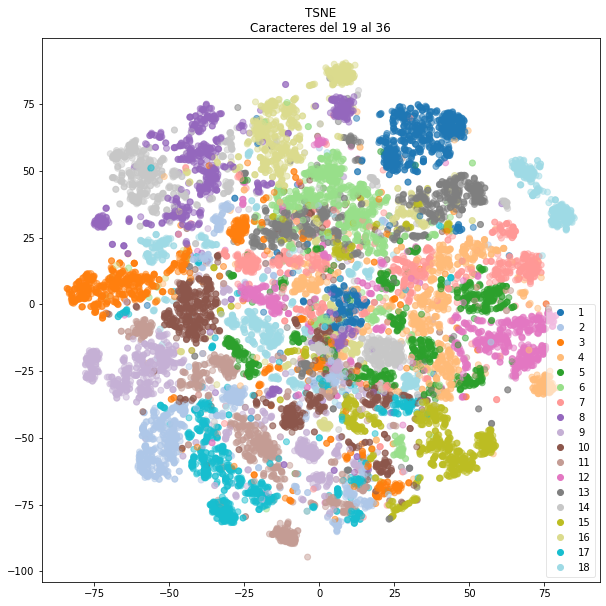
\includegraphics[width=77mm]{img/tsne2_sin_prep.png}}
	\subfigure[Con preprocesamiento]{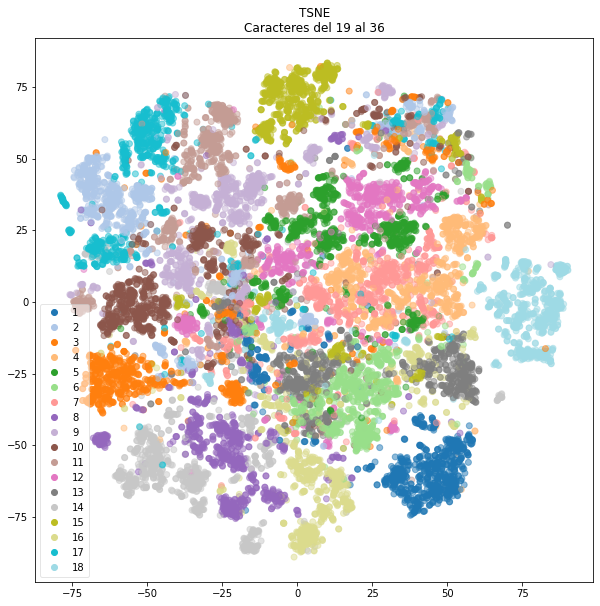
\includegraphics[width=77mm]{img/tsne2_con_prep.png}}
	\caption{Caracteres del 19 al 36}
	\label{fig:dimreduction2}
\end{figure}

\begin{figure}[H]
	\centering    
	\subfigure[Sin preprocesamiento]{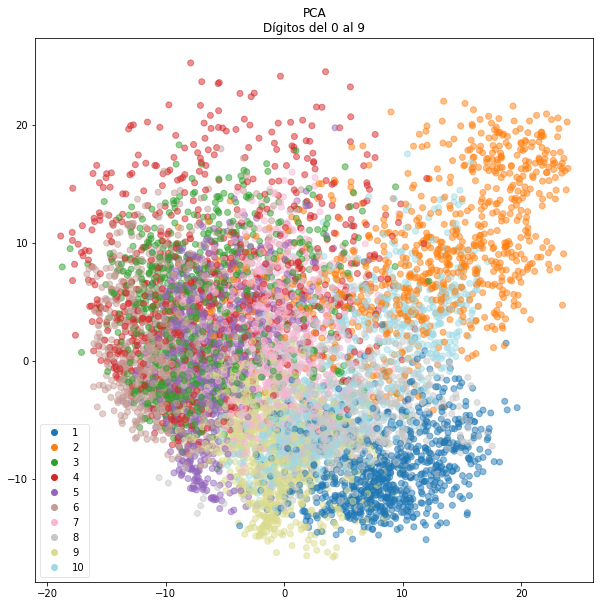
\includegraphics[width=77mm]{img/pca3_sin_prep.png}}
	\subfigure[Con preprocesamiento]{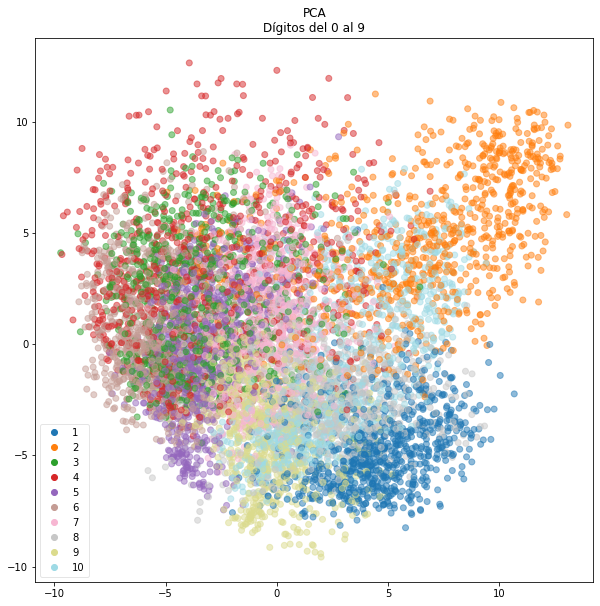
\includegraphics[width=77mm]{img/pca3_con_prep.png}}
	\subfigure[Sin preprocesamiento]{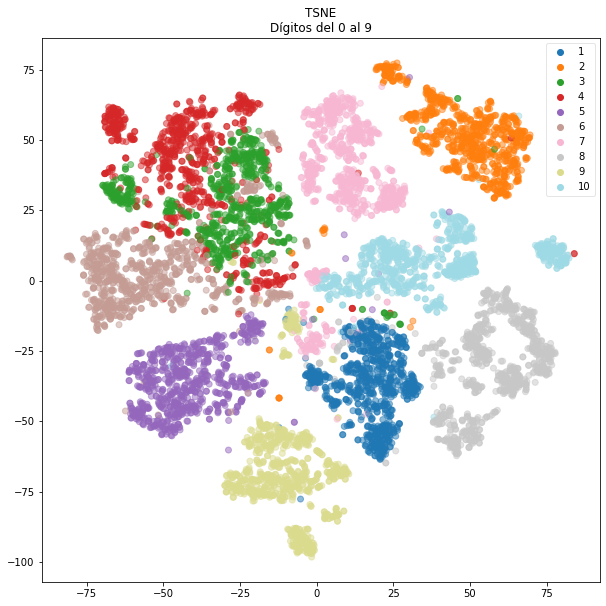
\includegraphics[width=77mm]{img/tsne3_sin_prep.png}}
	\subfigure[Con preprocesamiento]{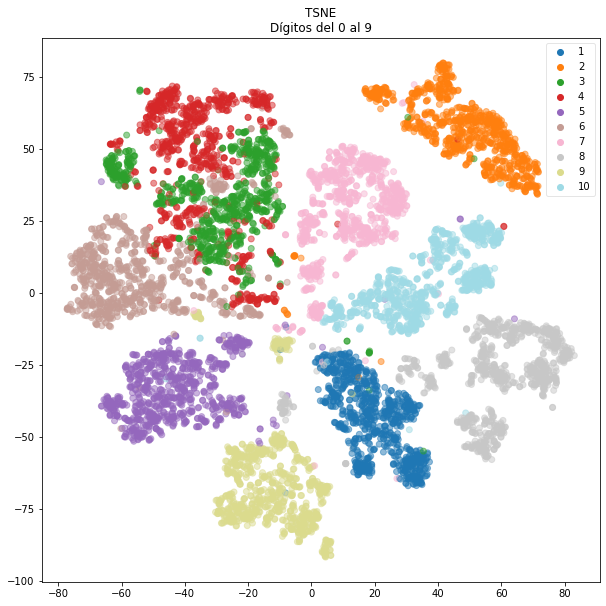
\includegraphics[width=77mm]{img/tsne3_con_prep.png}}
	\caption{Dígitos del 0 al 9}
	\label{fig:dimreduction3}
\end{figure}

En las visualizaciones obtenidas gracias a T-SNE podemos ver que los datos pertenecientes a una misma clase están en general más o menos agrupados y son cercanos entre sí. Sin embargo, también encontramos algunas clases superpuestas y algunos puntos dispersos. En las figuras que nos proporciona PCA apenas podemos distinguir unas clases de otras, no aportan mayor información. 

Por otro lado, notamos que las visualizaciones que se obtienen de los datos preprocesados son prácticamente iguales a las que se obtienen con los datos sin preprocesar, por lo que podríamos decir que no se pierde información por culpa del preprocesamiento. Es más, nos damos cuenta de que tras el preprocesamiento algunas clases se diferencian más claramente del resto, como es el caso del dígito 0, de modo que el aprendizaje será más sencillo. 

No obstante, debido a que estos gráficos son complicados de interpretar, no podemos usarlos para tomar decisiones importantes, como que el preprocesamiento es adecuado. Por ello, basamos nuestras decisiones en resultados empíricos. 


\underline{Referencias:}

 \href{https://towardsdatascience.com/pca-using-python-scikit-learn-e653f8989e60}{https://towardsdatascience.com/pca-using-python-scikit-learn-e653f8989e60}

 \href{https://towardsdatascience.com/visualising-high-dimensional-datasets-using-pca-and-t-sne-in-python-8ef87e7915b}{https://towardsdatascience.com/visualising-high-dimensional-datasets-using-pca-and-t-sne-in-python-8ef87e7915b}
 
 \href{https://www.displayr.com/using-t-sne-to-visualize-data-before-prediction/}{https://www.displayr.com/using-t-sne-to-visualize-data-before-prediction/}
 
\section{Métrica de error}

La métrica que usaremos para medir la bondad de los distintos modelos será la precisión, o \textit{accuracy}, que mide la proporción de puntos bien clasificados, proporcionando así valores entre 0 y 1. Puesto que el número de instancias pertenecientes a cada una de nuestras clases está balanceado, esta métrica es adecuada, y se utiliza con frecuencia para determinar la calidad de los modelos en los problemas de clasificación multietiqueta. Además, es simple y fácil de interpretar. 

Por otra parte, visualizaremos también la matriz de confusión para ver los resultados de manera gráfica.  Se trata de una matriz cuadrada de orden igual al número de clases, en la que la casilla $(i,j)$ contiene el número de instancias de la clase $i$ a los que el modelo ha asignado la clase $j$.  Así, el modelo será mejor cuanto mayores sean los valores en la diagonal y menores los valores fuera de esta, pues en la casilla $(i,i)$ se encuentra el número de ejemplos clasificados correctamente y en la $(i,j)$, con $i\neq j$, los ejemplos incorrectamente clasificados. 

Cabe notar que el \textit{accuracy} se calcula sumando los valores de la diagonal de la matriz de confusión, que será el número de instancias bien clasificadas, y dividiendo el resultado entre el número total de ejemplos. 



\section{Regresión Logística}

El modelo lineal que hemos elegido es Regresión Logística. Experimentalmente, se ha demostrado que para problemas con bastante ruido o en los que las clases se superponen, la maximización de la verosimilitud en la muestra da lugar a mejores soluciones que la optimización por separabilidad. Por ello, como no sabemos nada acerca de la separabilidad de los datos, consideramos que Regresión Logística es un modelo que nos permitirá alcanzar mejores resultados que otros modelos lineales para clasificación, como por ejemplo Perceptrón, el cual proporciona la mejor solución únicamente en el caso de datos separables linealmente. 

Otra razón para elegir este modelo frente a otros es su fácil adaptación a problemas de clasificación con más de dos clases, gracias a la Regresión Logística Multinomial.

Para implementar el modelo, usaremos \codeword{LogisticRegression} de \codeword{sklearn}. Este modelo cuenta con varios algoritmos de aprendizaje para ajustar nuestra hipótesis. De todos ellos, hemos decidido elegir SAGA por ser un algoritmo que maneja la pérdida multinomial y por tener una convergencia más rápida que otros algoritmos en problemas con conjuntos de datos de gran tamaño, como es nuestro caso. Este algoritmo es una mejora de otro llamado SAG (\textit{Stochastic Average Gradient}), que intenta mejorar sus ratios de convergencia. Ambos son una variación del gradiente descendente estocástico, que usan datos
de las iteraciones anteriores para intentar que la convergencia sea más rápida.

%Ambos están diseñados para minimizar una suma finita de funciones haciendo uso del gradiente, al igual que SGD.


\subsection{Función de pérdida y regularización}

En este caso, si $K$ es el número de clases y $N$ el tamaño de la muestra, la función de pérdida de este modelo es el error de entropía cruzada multinomial:

$$E(\textbf{w}_1,\dots,\textbf{w}_{K}) = -\frac{1}{N}\sum_{n=1}^{N} \sum_{k=1}^{K} y_{nk} \ln(\sigma(\textbf{w}_k^T \textbf{x}_n)) \qquad \text{donde } \sigma(t)=\frac{e^t}{1+e^t}$$

En la expresión anterior, $\textbf{x}_n$ es el vector de características asociado al punto n-ésimo de la muestra, $\textbf{w}_k$ es la fila k-ésima de la matriz de pesos, y 
las etiquetas $y_n$ del vector $\textbf{y}$ están codificadas como vectores one-hot, en los que $y_{nk} = 1$ si $y_n$ es la etiqueta asociada a la clase $k$ e $y_{nj} = 0$ para cualquier otro $j \neq k$.

Una vez calculados los pesos, el modelo hace uso de la regla de clasificación \textit{Softmax}, que obtiene un vector con las probabilidades que un elemento tiene de pertenecer a cada una de las clases. A continuación, este elemento será clasificado en la clase cuya probabilidad sea mayor.

$$Softmax(\textbf{x}_n) = \left(\frac{\exp(\textbf{w}_1 \textbf{x}_n)}{\sum_{k=1}^{K}\exp(\textbf{w}_k \textbf{x}_n)},\dots,\frac{\exp(\textbf{w}_{K} \textbf{x}_n)}{\sum_{k=1}^{K}\exp(\textbf{w}_k \textbf{x}_n)}\right)$$

En cuanto a la regularización, aplicaremos la de tipo \textit{Ridge}, o L2. Hemos elegido este tipo de regularización frente a \textit{Lasso} porque esta última tiende a anular algunos de los pesos en el ajuste del modelo, lo cual no nos conviene pues todas las características tienen una relevancia similar al ser de la misma naturaleza. Además, durante el preprocesamiento hemos intentado eliminar aquella información que pueda ser de menor utilidad para el modelo.

La regularización \textit{Ridge} añade la restricción $\|\textbf{w}\|^2 \leq C$, donde $C>0$ es una constante positiva y $\| \cdot \|$ es la norma de Frobenius. Esta restricción se refleja en la función de pérdida a través del error aumentado, que es el que se busca minimizar en este tipo de regularización:

$$E_{aug}(\textbf{w}) = E(\textbf{w}) + \frac{1}{C} \|\textbf{\textbf{w}}\|^2$$


\subsection{Estimación de hiperparámetros}

En todos los modelos, llevaremos a cabo una estimación de hiperparámetros mediante validación cruzada con 5 \textit{folds}.

%Dividiremos el conjunto de entrenamiento en 5 subconjuntos del mismo tamaño que mantengan la misma proporción entre clases y, fijando uno de ellos como conjunto de validación, ajustamos el modelo usando como conjunto de entrenamiento la unión de los 4 \textit{folds} restantes. Repetiremos esto para cada uno de los \textit{folds} y calcularemos el error medio cometido en los conjuntos de validación.

El único hiperparámetro que tenemos que estimar para este modelo es $C$, que denota la inversa de la intensidad de la regularización \textit{Ridge}. Como este hiperparámetro puede tomar valores en un rango de escalas muy amplio (desde valores muy cercanos a 0 hasta valores que tiendan a $+\infty$), primero aplicamos validación cruzada con $C$ tomando valores en el conjunto $\{10^{i/2} \ : \ i \in \{-6,-5,-4,\dots,2,3,4\} \}$. A continuación, tomaremos aquellos dos valores que obtengan mayor \textit{Accuracy} media y afinaremos la búsqueda en el intervalo que definen. Para hacer todo esto, hemos programado la función \codeword{findRange}. En la siguiente figura podemos ver la \textit{accuracy} media obtenida para cada uno de estos valores:

\begin{figure}[H]
    \centering
	\subfigure[Validación cruzada sobre $C$ (búsqueda del mejor intervalo)]{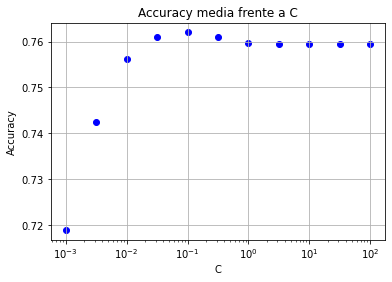
\includegraphics[width=77mm]{img/log_reg_cv1.png}}
	\label{fig:log_reg_cv1}
\end{figure}

Podemos ver que los dos valores con mayor \textit{accuracy} media son $C=10^{-1}$, con $0.76199$, y $C=10^{-1/2}$, con $0.76107$. Ahora, realizamos una búsqueda dicotómica en el intervalo $[10^{-1}, 10^{-1/2}]$ para afinar el valor de $C$. En cada iteración aplicaremos validación cruzada con $C$, tomamos el punto medio del intervalo actual y escogemos como siguiente intervalo aquel cuyos extremos son dicho punto medio y el extremo del intervalo actual que presente mayor \textit{accuracy}. Pararemos la búsqueda cuando la longitud del intervalo sea menor que un umbral, fijado en este caso a $10^{-2}$. Todo este procedimiento se ha realizado mediante la función \codeword{dichotomicSearch}, implementada por nosotros. En la siguiente figura podemos ver la \textit{accuracy} media obtenida por los valores considerados en la búsqueda:

\begin{figure}[H]
    \centering
	\subfigure[Validación cruzada sobre $C$ (primera búsqueda dicotómica)]{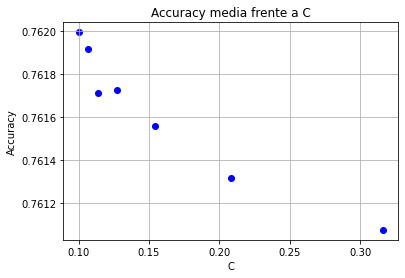
\includegraphics[width=77mm]{img/log_reg_cv2.png}}
	\label{fig:log_reg_cv2}
\end{figure}

Observamos que la mayor \textit{accuracy} media la arroja de nuevo el valor $C=10^{-1}$. Como este resultado se alcanza en el extremo del intervalo, hemos decidido ejecutar otra búsqueda dicotómica en el intervalo que se encuentra justo a su izquierda, es decir, en $[10^{-3/2},10^{-1}]$. Los resultados obtenidos se muestran en la siguiente figura:

\begin{figure}[H]
    \centering
	\subfigure[Validación cruzada sobre $C$ (segunda búsqueda dicotómica)]{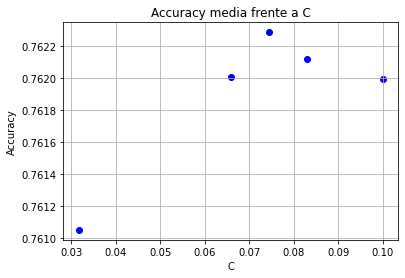
\includegraphics[width=77mm]{img/log_reg_cv3.png}}
	\label{fig:log_reg_cv3}
\end{figure}

Podemos ver que aquí sí mejoramos la mayor \textit{accuracy} media obtenida hasta el momento. Para \\$C=0.074358$ obtenemos un $0.76229$ de \textit{accuracy}. Éste será el valor que fijemos para este hiperparámetro.
Al ser un valor bajo, deducimos que la regularización considerada sí tiene efecto y mejora los resultados. 

\section{Perceptrón Multicapa}

El modelo de Perceptrón Multicapa que consideraremos tendrá una arquitectura de tres capas (dos capas ocultas y una de salida). Como se nos recomienda, fijaremos un número de neuronas por capa en el rango 50-100. Este hiperparámetro nos brinda la posibilidad de aumentar la complejidad para reducir el error dentro de la muestra y así obtener un sesgo bajo.

La implementación de \codeword{sklearn}, \codeword{MLPClassifier}, dispone de tres algoritmos distintos para la optimización de los pesos, de los cuales hemos seleccionado Adam. Este es un optimizador basado en gradiente descendente estocástico. Lo hemos elegido por estar recomendado (en la documentación de \textit{sklearn}) para conjuntos de datos relativamente grandes, como es nuestro caso. 

Otro parámetro importante que deberemos tener en cuenta es la función de activación, pues es el componente que aporta la no linealidad al modelo. En la implementación de \codeword{sklearn} se nos da a elegir entre tres activaciones distintas: ReLU, tangente hiperbólica y función logística. El tipo de activación que usemos será determinado de la misma forma que el resto de hiperparámetros. 

Este modelo es bastante flexible, tanto en lo relativo a su complejidad como en la regularización, pudiendo ajustarse de manera que presente bajo sesgo y baja varianza. Además, es adecuado para la clasificación multietiqueta, pues se adapta gracias a la regla softmax de la misma forma que lo hace regresión logística. Todo esto nos lleva a escoger MLP para ajustarlo a nuestro problema.

\subsection{Función de pérdida y Regularización}

La función de pérdida en este modelo es la misma que vimos en el caso de regresión logística multinomial, es decir, el error de entropía cruzada multinomial, y la predicción de las clases también se lleva a cabo de la misma forma, usando la función softmax. 

Si la complejidad del modelo llega a ser excesiva, puede llevarnos a sobreajuste. Para evitarlo, aplicaremos dos mecanismos de regularización que nos permitan alcanzar un mayor equilibrio entre sesgo y varianza.

El primero de ellos será regularización de tipo \textit{Ridge}, ya explicada en el caso de regresión logística. Para aplicarla correctamente, estimaremos el valor de un hiperparámetro $\alpha>0$, que se corresponde con la inversa del parámetro $C$ que vimos para la regularización en Regresión Logística.

El segundo mecanismo que probaremos será \textit{Early Stopping}. Por defecto, el criterio de parada sin  \textit{Early Stopping} consiste en parar el entrenamiento cuando el número de iteraciones consecutivas en las que el modelo no mejora el error en entrenamiento más de $10^{-4}$ es superior a 10. Si aplicamos \textit{Early Stopping}, se separará un 10\% del conjunto de entrenamiento, que será destinado a validación, de forma que, al ajustar el modelo, el error que se tendrá en cuenta en el criterio de parada será el del conjunto de validación.


\subsection{Estimación de hiperparámetros}

Necesitamos estimar cuatro hiperparámetros:

\begin{itemize}
    \item Número de neuronas de las capas ocultas: entre 50 y 100
    \item Tipo de activación: ReLU, tangente hiperbólica o función logística
    \item Parámetro de regularización \textit{Ridge}: $\alpha \in ]0,+\infty[$
    \item Early Stopping: sí o no
\end{itemize}

Empezamos estimando el número de neuronas junto con el tipo de activación. Para ello, aplicamos tres búsquedas dicotómicas en el rango de valores 50-100 para cada una de las tres activaciones. Los resultados obtenidos en cada una de ellas se encuentran en la siguiente figura:

\begin{figure}[H]
    \centering
	\subfigure[Búsqueda dicotómica sobre el número de neuronas para cada tipo de activación]{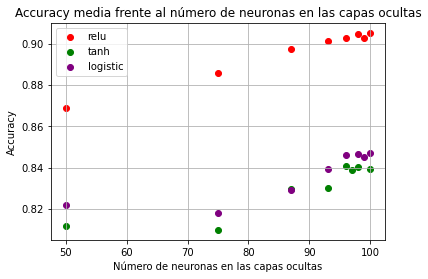
\includegraphics[width=77mm]{img/mlp_cv1.png}}
	\label{fig:mlp_cv1}
\end{figure}

Observamos que la mayor \textit{accuracy} media se alcanza con 100 neuronas por capa oculta y activación ReLU, luego fijamos estos valores en nuestro modelo.

A continuación, estimamos el valor del parámetro de regularización $\alpha$. En este caso, procederemos de forma análoga a como se hizo en Regresión Logística. Primero, realizamos una búsqueda a distintas escalas usando el rango de valores $\{10^{i/2} \ : \ i \in \{-10,-9,-8,\dots,0,1,2\} \}$.  En la siguiente figura podemos ver la \textit{accuracy} media obtenida para cada uno de estos valores:

\begin{figure}[H]
    \centering
	\subfigure[Validación cruzada sobre $\alpha$ (búsqueda del intervalo)]{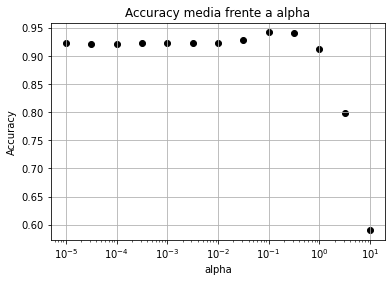
\includegraphics[width=77mm]{img/mlp_cv2.png}}
	\label{fig:mlp_cv2}
\end{figure}

Podemos ver que los dos valores con mayor \textit{accuracy} media son $\alpha=10^{-1}$, con $0.94160$, y $\alpha=10^{-1/2}$, con $0.94027$. Ahora, realizamos una búsqueda dicotómica en el intervalo $[10^{-1}, 10^{-1/2}]$ para afinar el valor de $\alpha$. En la siguiente figura podemos ver la \textit{accuracy} media obtenida por los valores considerados en la búsqueda:

\begin{figure}[H]
    \centering
	\subfigure[Validación cruzada sobre $\alpha$ (búsqueda dicotómica)]{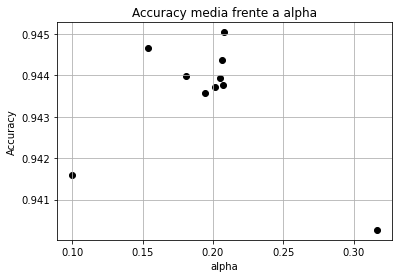
\includegraphics[width=77mm]{img/mlp_cv3.png}}
	\label{fig:mlp_cv3}
\end{figure}

Observamos que la mayor \textit{Accuracy} media la ofrece el valor $\alpha=0.20811$ con un $0.94504$.

Por último, estudiamos el impacto de \textit{Early Stopping} con la configuración de hiperparámetros obtenida hasta el momento. Al aplicarlo, obtenemos una \textit{accuracy} media de $0.93198$, inferior a la obtenida anteriormente sin aplicar \textit{Early Stopping}. Por tanto, decidimos no aplicar este mecanismo de regularización.

La configuración final de hiperparámetros es la siguiente:

\begin{itemize}
    \item Número de neuronas de las capas ocultas: 100
    \item Tipo de activación: ReLU
    \item Parámetro de regularización \textit{Ridge}: $\alpha=0.20811$ 
    \item Early Stopping: no
\end{itemize}






\section{Random Forest}

Este modelo construye un cierto número de árboles de decisión (\codeword{n_estimators}) y asigna a cada ejemplo la clase que tiene el voto mayoritario de entre todos los árboles construidos. Cada árbol se contruye usando una cierta proporción del número total de instancias del conjunto de entrenamiento (\codeword{max_samples}) y un subconjunto de las características de las que se parte (\codeword{max_features}). Al usar sólo un subconjunto de las características, los distintos árboles construidos tendrán un grado bajo de correlación, de modo que se reduce la varianza del modelo. Tomamos como \codeword{max_features} la raíz cuadrada del número total de características, que es un valor adecuado como se vio en clase de teoría. Además, es claro que cuántos más instancias se usen para construir cada uno de los árboles, mejores serán las predicciones de estos, por lo que consideramos toda la muestra para el entrenamiento de cada árbol  (\lstinline{max_samples=X.shape[0]}). Estos valores de los parámetros son los que trae por defecto \codeword{RandomForestClassifier} de \textit{sklearn}. 

Los árboles de decisión son un modelo fácil de interpretar y apropiado para la clasificación multietiqueta, pues se asigna fácilmente una clase a cada nodo hoja. Además, al combinar varios árboles usando Random Forest se reduce la varianza que cada uno de ellos presenta por separado y, si no podamos los árboles, estos tienen bajo sesgo. Por tanto, tenemos un modelo con bajo sesgo y baja varianza. Estos hechos nos llevan a elegir Random Forest como uno de los modelos a usar para nuestro problema de aprendizaje. 

\subsection{Función de pérdida y regularización}

En random forest, la función de pérdida a minimizar en cada uno de los árboles es:

\[C_{\alpha}(T) = \sum\limits_{m=1}^{|T|} N_mQ_m(T) + \alpha|T|\] donde $|T|$
es el número de nodos terminales del árbol $T$, $N_m$ es el número de
ejemplos en el nodo terminal $m$ y $Q_m(T)$ es la impureza del nodo terminal $m$. Tenemos también el parámetro $\alpha$, que es un coeficiente que determina la penalización por la complejidad del árbol $T$, la cual se mide en función del número de hojas, de manera que cuantos más nodos terminales tenga el árbol mayor será su complejidad. Así,  $\alpha$ puede ser visto como un parámetro de regularización. 

Para medir la impureza de un nodo, $Q_m(T)$,
consideramos el índice de Gini:

\[Q_m(T) = \sum\limits_{k=1}^{K} \hat p_{mk}(1 - \hat p_{mk})\] donde
$\hat p_{mk}$ es la proporción de ejemplos de la clase $k$ que hay en el nodo $m$.

Esta medida es la más frecuente, aunque proporciona resultados similares a otras,  como por ejemplo la entropía, según lo comentado en clase de teoría.

\subsection{Estimación de hiperparámetros}

Entre los parámetros de este modelo se encuentran los asociados a cada uno de los árboles, como son el criterio usado para medir la calidad de cada ramificación (nos quedamos con \textit{GINI} como ya hemos comentado), la profundidad máxima del árbol, el mínimo número de ejemplos que debe haber en un nodo para dividirlo, el mínimo número de ejemplos que debe haber en un nodo hoja, máximo número de nodos hojas, y demás parámetros usados para el \textit{early stopping} en la construcción del árbol. Puesto que esta estrategia no es muy frecuente, requiere ajuste de numerosos parámetros y además introduce un sesgo en cada árbol, optamos por dejar estos parámetros con los valores por defecto, que son los que permiten a cada árbol desarrollese completamente. 

Otro parámetro que ofrece \codeword{RandomForestClassifier} es \codeword{bootstrap}, que lo dejamos a su valor por defecto que es True, pues en otro caso se usarían todas las características para construir cada árbol, haciendo que estos estén altamente correlados. 

Sin embargo, el parámetro más importante a ajustar es el número de árboles que se construyen, \codeword{n_estimators}, por lo que es el hiperparámetro que vamos a configurar. Además, para paliar el posible sobreajuste que pudiera haber, ajustamos el parámetro  $\alpha$ (\codeword{ccp_alpha}) .

Para determinar el número de árboles que ofrece el mejor valor de accuracy en validación cruzada usamos la función \codeword{dichotomicSearch}(ya explicada) con 5 particiones para que los resultados sean fiables. Tomamos el intervaloo $[100,300]$ para aplicar la búsqueda dicotómica, y obtenemos que el mejor valor para el número de árboles es 290, con un accuracy de 0.92263.

Para tener una idea visual de los resultados los mostramos en una gráfica en función del número de árboles: 

\begin{figure}[H]
	\subfigure[Gráfico sin ampliar]{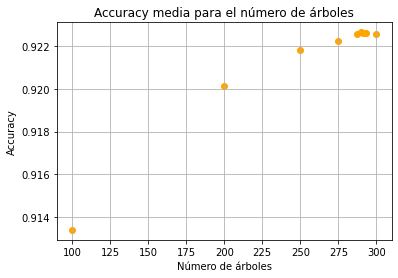
\includegraphics[width=77mm]{img/rf_numarboles.png}}
	\subfigure[Gráfico ampliado]{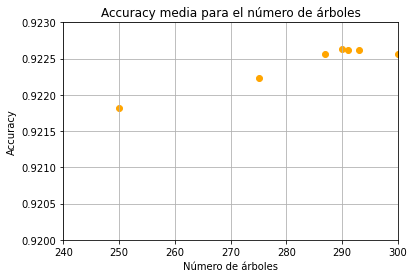
\includegraphics[width=77mm]{img/rf_numarboles2.png}}
	\label{fig:num_arboles}
\end{figure}

Por otro lado, para configurar el valor del parámetro $\alpha$ usamos la función \codeword{findRange}, con 6 valores entre $10^{-6}$ y $10^{-1}$, esto es, $10^{-6}, 10^{-5}, 10^{-4},...,0.1$, y nos damos cuenta que el accuracy en validación cruzada disminuye conforme aumentamos el valor de alpha:

\begin{figure}[H]
    \centering
    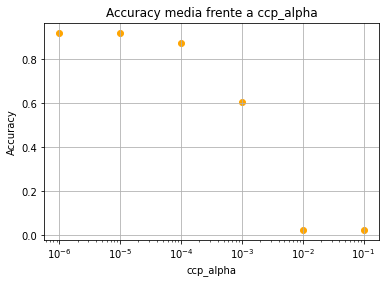
\includegraphics[width=77mm]{img/rf_alpha.png}
	\label{fig:ccp_alpha}
\end{figure}

Por lo tanto, decidimos tomar \lstinline{ccp_alpha=0}, que es el valor por defecto. Esto nos hace pensar que el criterio de \textit{cost-complexity} empleado a modo de regularización no es adecuado en nuestro caso, o que el sobreajuste no es un problema a tener en cuenta aquí. De hecho, puesto que Random Forest presenta una varianza y sesgo bajos, como ya hemos explicado, el error de generalización también será bajo, y dependerá principalmente del ruido estocástico de los datos.

\underline{Referencias:}

\href{https://scikit-learn.org/stable/modules/tree.html#minimal-cost-complexity-pruning}{https://scikit-learn.org/stable/modules/tree.html}

\href{https://scikit-learn.org/stable/modules/generated/sklearn.ensemble.RandomForestClassifier.html}{https://scikit-learn.org/stable/modules/generated/sklearn.ensemble.RandomForestClassifier.html}

\section{Modelos extra}

\subsection{Support Vector Machines}

Una máquina de soporte de vectores construye un hiperplano separador en un espacio con alta dimensionalidad, el cual se usa para la clasificación. Este hiperplano se intenta buscar lo más 'grueso' posible, es decir, que maximice la distancia entre los puntos más cercanos de dos clases diferentes, pues la dimesión VC es menor cuanto más grueso sea el hiperplano separador (el margen entre dos clases), de manera que el error de generalización también disminuye al aumentar el ancho del margen.   

El enfoque usado será SVM-Soft, es decir, se acepta una cierta violación del margen de separación para cada punto de la muestra. Así, se permite que algunos puntos estén mal clasificados o dentro del margen de separación, de manera que este enfoque es más robusto al ruido y es menos probable que incurra en sobreajuste. 

En cuanto al kernel, tomamos el kernel gaussiano RBF:

$$K(x,x')=exp(-\gamma\|x-x'\|^2),\hspace{2mm} x,x'\in \mathbb{R}^d$$

por ser uno de los más usados, potente y sólo tiene un parámetro que ajustar, que es $\gamma>0$. 

Elegimos SVM porque proporciona la solución óptima, en el sentido de que minimiza la dimensión de VC, en el caso en que los datos sean separables. Si no son separables, lo cual ocurre normalmente,\\ SVM-Soft también encuentra la solución de menor error de generalización para cada valor del parámetro de regularización C, lo cual no está garantizado para otros modelos. 

Este modelo está diseñado para la clasificación binaria, pero nuestro problema tiene múltiples clases. Sin embargo, gracias a las estrategias one-vs-rest y one-vs-one, las SVM se pueden usar también para la clasificación multietiqueta. Consideraremos el enfoque one-vs-rest, pues requiere el entrenamiento de tantos clasificadores como clases tengamos (46), mientras que one-vs-one necesita entrenar $num\_clases\frac{num\_clases - 1}{2}$ (1035 en nuestro caso), de manera que este último es mucho más costoso y requiere un mayor tiempo de cómputo. El primero es el valor por defecto en \textit{scikit-learn}. 

\subsubsection{Función de pérdida y regularización} 

Dado un conjunto de instancias $x_n\in\mathbb{R}^d, n=1,2,...,N$ (N es el número de muestras de entrenamiento y $d$ el número de características) distribuidas en dos clases y un vector de etiquetas $y\in \{-1,1\}^N$, se intenta resolver el siguiente problema de optimización (problema dual):
\begin{align*}
\min\limits_{\alpha}\frac{1}{2}\alpha^TQ\alpha - e^T\alpha\\
\text{Sujeto a: } y^T \alpha =0\\
 0\leq \alpha_n \leq C \text{ para } n=1,...,N
\end{align*}

siendo $e^T=(1,.^{N)}..,1)$ y Q  una matriz de orden $N\times N$ semidefinida positiva con $Q_{ij}=y_iy_jK(x_i,x_j)$.

La hipótesis final será 
$$g(x)=sign\big( \sum_{\alpha_n^{*}>0}y_n\alpha_n^{*}K(x_n,x)+b^{*} \big)$$
donde $\alpha_n^{*}$ y $b^{*}$ son la solución al problema de optimización. 

Los coeficientes $\alpha_n^{*}$ están acotados superiormente por el parámetro C. Este es el peso de la penalización porque un punto quede dentro del margen de separación o esté mal clasficado. Por lo tanto, cuanto menor sea el parámetro C más peso tendrá la regularicación y menos la violación del margen.  


\subsubsection{Estimación de hiperparámetros}

Como hemos ido comentando, los dos hiperparámetros más importantes que tenemos que estimar son el valor de $C$ y del coeficiente $\gamma$ del kernel RBF. 

Empezamos fijando el valor de $\gamma$ al que tiene por defecto \textit{scikit-learn} que es $ \frac{1}{n\_features\cdot Var(X)}$, y estimamos $C$ usando la función \codeword{findRange} con $0.01,0.1,1,10,100$ (pues se nos pide una precisión de 2 cifras en los parámetros para SVM). El valor que ofrece mejores resultados ha sido $C=100$, con un Accuracy media de validación cruzada de 0.96148

\begin{figure}[H]
    \centering
    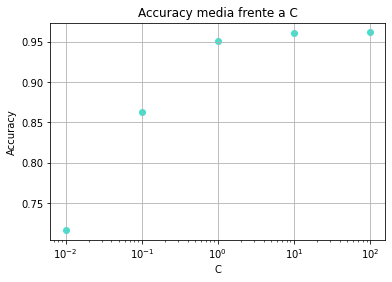
\includegraphics[width=77mm]{img/svm_C.png}
	\label{fig:C}
\end{figure}

Del mismo modo, para $\gamma$ probamos los valores $0.001,0.01,0.1,1,10$ y obtenemos los resultados que se presentan a continuación de manera gráfica: 

\begin{figure}[H]
    \centering
    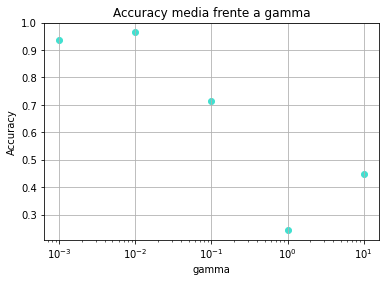
\includegraphics[width=77mm]{img/svm_gamma.png}
	\label{fig:gamma}
\end{figure}

Vemos que el valor con mejor \textit{accuracy} es $0.01$, con 0.96434.

El alto valor que se obtiene para el parámetro C indica que la regularización a penas tiene efecto, pues se penaliza mucho el hecho de que un punto quede dentro del 'pasillo', de modo que habrá pocos puntos que violen el margen. 

Por su parte, el parámetro $\gamma$ determina la amplitud del kernel Gaussiano, de modo que cuanto mayor sea $\gamma$ más 'estrechas' serán las funciones Gaussianas, dando lugar a hipótesis complejas y, por lo tanto, a una mayor tendencia al sobreajuste. El valor que obtenemos es bajo, lo que indica que las hipótesis no son demasiado complejas. Este bajo valor de $\gamma$ compensa el alto valor de $C$, de modo que lo que se tiene son hipótesis no muy complejas pero pasillos estrechos.  

\underline{Referencias}:

\href{https://scikit-learn.org/stable/modules/generated/sklearn.svm.SVC.html}{https://scikit-learn.org/stable/modules/generated/sklearn.svm.SVC.html}

\href{https://scikit-learn.org/stable/modules/svm.html}{https://scikit-learn.org/stable/modules/svm.html}

\subsection{Red de funciones de base radial}

Podemos ver este modelo como un tipo de perceptrón multicapa con tres capas (entrada, salida y capa oculta), donde la función de activación es una función de base radial. En concreto, consideramos la función: 

$$\Phi(z)=e^{-\frac{1}{2}z^2}$$

$\Phi(\|x-x_n\|)$ determina la influencia que el punto $x_n$ tiene sobre el punto $x$. Esta decrece gradualmente conforme aumenta la distancia entre  $x_n$ y $x$. 

Una hipótesis de la clase de funciones de este modelo tiene la siguiente forma:

$$ h(x)=w_0 + \sum_{i=1}^k w_i\Phi\Big( \frac{\|x-\mu_i\|}{r}\Big) $$

donde $\mu_i, i=1,...,k$, son centros de ciertos clusters dentro del conjunto de datos, r es un parámetro de escala que determina la \textit{unidad} de medida de la distancia entre los puntos y $w$ es el vector de pesos. 

El valor de $k$ determina el tamaño del conjunto de hipótesis. Este es el número de centros, o clusters, que se desea considerar. Cuanto mayor sea k, más propenso será el modelo al sobreajuste y, si k es muy pequeño, puede producirse underfitting. Por su parte, $r$ determina la complejidad de una hipótesis. 

Tomamos $$r=\frac{R}{k^{1/d}}$$ donde d es el número de características, y $R=\max_{i,j}\|x_i-x_j\|$ es el \textit{diámetro} de los datos. Este es el valor de $r$ recomendado en \textit{Learning from data, Similarity Based Methods, pg.29}. Al calcular este diámetro sobre el conjunto de datos preprocesados (sin aplicarle estandarización) usando la función programada por nosotros mismos \codeword{computeR}, obtenemos un valor de $R=2677.163$.

Para este modelo no es necesario aplicar ningún tipo de normalización previa a los datos, como hemos hecho con \codeword{StandardScaler} para el resto de modelos. Esto es debido al parámetro de escala $r$, que, gracias al cálculo del diámetro $R$, se encarga de escalar las distancias entre los datos de la manera más adecuada.


El valor de $k$ lo estimaremos a continuación, mediante validación cruzada. 

Para cada valor de k, los centroides, $\mu_i, i=1,...,k$, los calcularemos mediante el algoritmo de $k-means$, haciendo uso de \codeword{KMeans} de \textit{sklearn}.

Dadas las similitudes de este modelo con el perceptrón multicapa y con SVM con kernel Gaussiano RBF, escogemos RBF-Network como segundo modelo extra para comparar los resultados del mismo con los obtenidos con MLP y SVM. 

\subsubsection{Función de pérdida y regularización}

Consideramos la matriz $Z$, donde, para cada $n=0,...,N-1$ (N es el número de muestras en el conjunto de datos) $Z_{n,0}=1$ y $Z_{n,j}=\Phi\Big(\frac{\|x_n-\mu_j\|}{r}\Big), j= 1,...,k$, y ajustamos el modelo lineal $Zw$ al vector de etiquetas $y$ (estas se codifican a vectores one-hot). Para ello, usamos el algoritmo de la pseudo-inversa, donde la función de pérdida a minimizar es el error cuadrático medio, que nos da un valor cerrado para los pesos, $w$. 

Para predecir la clase de un punto desconocido $x$, calculamos el vector cuya componente j-ésima viene dada por  $\Phi\Big(\frac{\|x-\mu_j\|}{r}\Big), j = 1,...,k$, y en la primera posición tiene un 1. A continuación, se multiplica dicho vector por los pesos, calculados mediante el algoritmo de la pseudoinverda, y se le asigna al punto $x$ la clase correspondiente a la posición en el vector resultante que presenta el valor más alto (habrá 46 posiciones, una por cada clase). 

No añadimos restricciones a los valores de los pesos (regularización), pues eligiendo un valor de k adecuado (no demasiado grande), podemos evitar en cierta medida el sobreajuste. 

\textbf{Nota}.

Este modelo no se encuentra implementado como tal en la librería de \textit{sklearn} (y no hemos conseguido encontrar ninguna otra donde esté), de modo que hemos tomado la implementación que se propone en \href{https://towardsdatascience.com/most-effective-way-to-implement-radial-basis-function-neural-network-for-classification-problem-33c467803319}{towardsdatascience.com/most-effective-way-to-implement-radial-basis-function-neural-network-for-classification-problem}, modificando el código para adaptarlo al modelo que se ha visto en clase de teoría y para intentar hacerlo algo más eficiente (por ejemplo usando \codeword{KMeans} de \textit{sklearn} en lugar de la implementación que ahí se propone).

\subsubsection{Estimación de hiperparámetros}

El único hiperparámetro que debemos ajustar, según lo comentado anteriormente, es el número de clusters, $k$. Para ello usaremos validación cruzada. 

Debemos implementar nosotros mismos el código de validación cruzada para aplicarlo a RBF-Network, pues, como ya hemos dicho, este no es un modelo de sklearn y no está adaptado para usarlo con la función \codeword{cross_val_score}. Implementamos así la función \codeword{cross_val_rbf}.

Consideramos otra función, \codeword{findBestK}, que se encarga de, dada una lista de parámetros, aplicar validación cruzada con tres particiones para cada uno de los valores del parámetro k de esa lista, devolver los valores de accuracy medios obtenidos y visualizar los resultados en un gráfico. Tomamos tres particiones y no cinco como venimos haciendo hasta ahora porque el código es bastante lento al no estar optimizado ni paralelizado, de modo que considerar más particiones supondría mucho más tiempo de ejecución.

Así, le damos a $k$ los valores 100, 500, 1000 y 1500, pues, dado el alto número de clases de las que disponemos, considerar un menor número de clusters nos lleva a underfitting y, con un K mayor a 1500 el tiempo de ejecución se vuelve muy elevado. Los resultados que se obtienen se muestran en la siguiente figura: 

\begin{figure}[H]
    \centering
	\subfigure{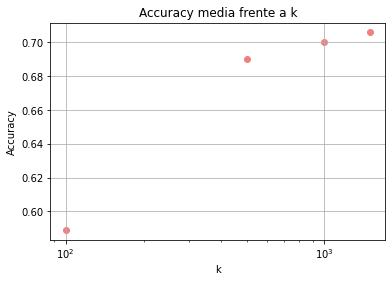
\includegraphics[width=77mm]{img/rbf_k.png}}
	\label{fig:rbf}
\end{figure}


Vemos que el accuracy mejora al aumentar el valor de $k$, de manera que optamos por tomar $k=1500$, con el que obtenemos un accuracy media en las tres particiones de validación cruzada de 0.70581. 


\section{Selección de la mejor hipótesis}

Para determinar cuál de las hipótesis estudiadas es mejor, usaremos el error de validación (o \textit{accuracy} en nuestro caso, en vez de error) sobre un conjunto de validación que separamos del conjunto de entrenamiento original y supone el 20\% del mismo, tal y como comentamos en el apartado correspondiente. Así, entrenamos nuestros modelos, con los hiperparámetros ya ajustados, en el 80\% del conjunto de entrenamiento original, y los validamos en el conjunto de validación. No usamos validación cruzada puesto que, dado el elevado número de instancias de las que disponemos, esta se vuelve computacionalmente muy costosa, y el tamaño del conjunto de validación es suficientemente grande como para ser representativo. En la siguiente tabla se muestran los resultados obtenidos por cada modelo:

\begin{table}[H]
	\centering
    \begin{tabular}{|l|c|c|}
    \hline
    \multicolumn{1}{|c|}{\textbf{Modelos}} & \multicolumn{1}{l|}{\textbf{Accuracy en entrenamiento}} & \textbf{Accuracy en validación} \\ \hline
    Regresión Logística                    & 0.77417                                                 & 0.74815                         \\ \hline
    Perceptrón Multicapa                   & 0.98911                                                 & 0.93939                         \\ \hline
    Random Forest                          & 1                                                       & 0.91905                         \\ \hline
    SVM Gaussian-RBF                       & 1                                                       & 0.96183                         \\ \hline
    RBF-Network                            & 0.7137                                                & 0.70511                      \\ \hline
    \end{tabular}
	\caption{\textit{Accuracy} obtenida por cada modelo en validación}
	\label{table:validacion}
\end{table}

Como era esperable, Regresión Logística (nuestro único modelo lineal) obtiene resultados bajos de \textit{accuracy}, ya que la dificultad del problema requiere de modelos con mayor complejidad. De hecho, el error en el conjunto de entrenamiento también es alto, de manera que el modelo no es suficientemente complejo como para ajustarse bien al conjunto de entrenamiento.  

El modelo que presenta el valor de accuracy más alta es SVM con el kernel gaussiano, seguido del perceptrón multicapa y Random Forest.  

Tanto Random Forest como SVM se ajustan perfectamente al conjunto de entrenamiento, mientras que MLP no llega a ajustarse completamente, pero el error es muy bajo.  Por lo tanto, podemos decir que estos modelos son lo suficientemente complejos como para explicar toda la variabilidad de la muestra. No obstante, podemos ver que el error de generalización obtenido no es muy grande, de modo que el sobreajuste no tiene demasiado efecto. 

Por su parte, las redes de funciones de base radial son las que ofrecen los peores resultados, 
incluso en el conjunto de entrenamiento. Esto nos lleva a pensar que se produce underfitting, y el modelo no es lo suficientemente complejo como para ajustarse al conjunto de datos. Quizás si hubiéramos considerado un valor de k más elevado los resultados habrían sido mejores, pues ya vimos al ajustar este parámetro que los resultados mejoraban cuando este crecía. Sin embargo, puesto que con un mayor valor de k el tiempo de ejecución se dispara, no hemos podido considerar valores mayores. También es posible que si hubiéramos configurado el parámetro $r$ los resultados mejoraran. 
Por otra parte, como este modelo está implementado por nosotros, no dispone de la potencia y eficiencia que presentan los demás modelos de \textit{sklearn}, de ahí que los resultados sean peores, y no podamos ajustar sus parámetros de manera más fina. 

Por lo tanto, teniendo en cuenta los resultados que cada uno de los modelos presenta sobre el conjunto de validación, elegiríamos las \textbf{SVM con kernel gaussiano RBF} para ajustar nuestra hipótesis final sobre todo el conjunto de entrenamiento y evaluar los resultados sobre el conjunto de test. 

\section{Evaluación de los modelos sobre el conjunto de test}

En una situación real, el conjunto de test lo usaríamos para evaluar únicamente la calidad de la mejor hipótesis anteriormente seleccionada. Sin embargo, en este proyecto evaluaremos el desempeño de todos los modelos ajustados con un interés puramente académico. Insistimos en que el conjunto de test nunca debe ser usado para seleccionar la mejor hipótesis.

Hemos entrenado cada uno de los modelos con todos los datos del conjunto de entrenamiento original. A continuación, los hemos evaluado sobre ambos conjuntos, de entrenamiento y de test. La accuracy obtenida por cada uno de ellos puede verse en la siguiente tabla.

\begin{table}[H]
	\centering
    \begin{tabular}{|l|c|c|}
    \hline
    \multicolumn{1}{|c|}{\textbf{Modelos}} & \multicolumn{1}{l|}{\textbf{Accuracy en entrenamiento}} & \textbf{Accuracy en test} \\ \hline
    Regresión Logística                    & 0.77207                                                 & 0.75841                   \\ \hline
    Perceptrón Multicapa                   & 0.98738                                                 & 0.95167                   \\ \hline
    Random Forest                          & 1                                                       & 0.93094                   \\ \hline
    SVM Gaussian-RBF                       & 1                                                       & 0.96993                   \\ \hline
    RBF-Network                            & 0.7155                                               & 0.71311                  \\ \hline
    \end{tabular}
	\caption{\textit{Accuracy} obtenida por cada modelo en test}
	\label{table:test}
\end{table}

Vemos que, al tener un conjunto de entrenamiento de mayor tamaño, los resultados sobre el conjunto de test mejoran con respecto a los obtenidos en validación, pues ahora se dispone de más datos con los que entrenar los modelos. 

Las conclusiones que sacamos a partir de los resultados en el conjunto de validación, se siguen cumpliendo para los resultados en el conjunto de test. 

Sabemos que $E_{test}$ proporciona una buena estimación para el error fuera de la muestra. De hecho es un estimador
insesgado. Por lo tanto, podemos considerar que el error fuera de la muestra para nuestra mejor hipótesis es  $E_{out}\approx E_{test}=0.96993$


A continuación, mostramos las matrices de confusión de todos los modelos:

\begin{figure}[H]
    \centering
	\subfigure[Regresión Logística]{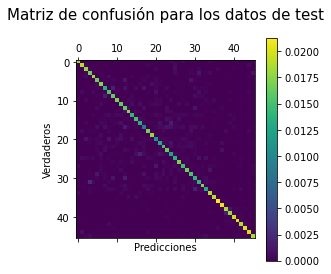
\includegraphics[width=77mm]{img/log_reg_mat_conf.png}}
	\subfigure[Perceptrón Multicapa]{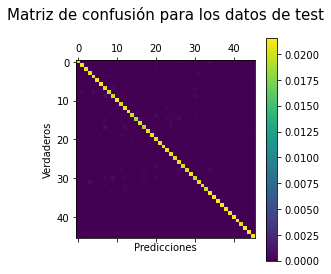
\includegraphics[width=77mm]{img/mlp_mat_conf.png}}
	\subfigure[Random Forest]{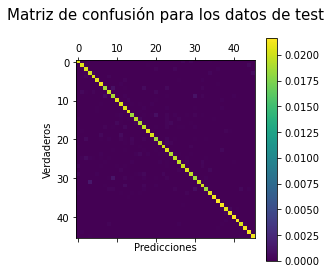
\includegraphics[width=77mm]{img/rf_mat_conf.png}}
	\subfigure[SVM Gaussian-RBF]{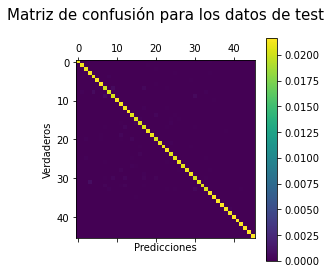
\includegraphics[width=77mm]{img/svm_mat_conf.png}}
	\subfigure[RBF-Network]{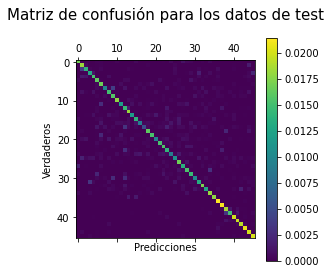
\includegraphics[width=77mm]{img/confusion_rbf.png}}
	\caption{Matrices de confusión}
	\label{fig:matrices_confusion}
\end{figure}


Podemos ver que las matrices de confusión correspondientes a SVM y MLP son prácticamente diagonales, lo cual era esparable por los valores de accuracy    obtenidos sobre el conjunto de test. 

Por otra parte, notamos que la matriz de Random Forest presenta algunas instancias fuera de la diagonal, pues el accuracy de este era algo inferior. Estas instancias se corresponden con datos del conjunto de test que no han sido clasificadas correctamente por el modelo. 

Las matrices de Regresión Logística y RBF-Network, al ser los modelos que obtienen el peor ajuste, presentan bastantes más ejemplos fuera de la diagonal principal, como era de esperar.


\section{Conclusiones}

Según se indica en el enlace \href{https://archive.ics.uci.edu/ml/datasets/Devanagari+Handwritten+Character+Dataset}{https://archive.ics.uci.edu/ml/datasets/Devanagari+Handwritten+Character+Dataset}, de donde hemos descargado nuestros datos, el mejor valor de accuracy obtenido sobre el conjunto de datos de test es de 98.47\%, presentado en el artículo \href{https://ieeexplore.ieee.org/stamp/stamp.jsp?tp=&arnumber=7400041}{Deep learning based large scale handwritten Devanagari character recognition}.

Este valor supera los resultados que hemos obtenido nosotros. Sin embargo, se utilizan técnicas de Deep Learning con Redes Neuronales Convolucionales para obtener el valor de accuracy más alto y las CNN son el modelo que presenta los mejores resultados en los problemas con imágenes. 

En nuestro estudio no hemos considerado este tipo de redes neuronales y, sin embargo, gracias al preprocesamiento de los datos y el ajuste de hiperparámetros llevado a cabo, hemos conseguido superar el 90\% de accuracy sobre el conjunto de test para la mayoría de los modelos. De hecho, con SVM (nuestro mejor modelo) conseguimos casi un 97\%, bastante cerca al mejor valor alcanzado (98.47\%). 

Por lo tanto, teniendo en cuenta que no hemos usado los mejores modelos que existen para el tipo de problema al que nos enfrentamos, podemos decir que hemos logrado obtener los mejores resultados alcanzables con casi todos nuestros modelos y estos son bastante satisfactorios. 

 
\newpage
\section{Apéndice: Instrucciones para la ejecución del código}

En la consigna de la UGR hemos subido los archivos con extensión \codeword{.npy} relativos al conjunto de entrenamiento (\codeword{x_train.npy} y \codeword{y_train.npy}) y al de test (\codeword{x_test.npy} y \codeword{y_test.npy}). Estos archivos son el resultado de leer las imágenes con la función \codeword{loadDataset}. Entregamos estos archivos para que se puedan reproducir los resultados que hemos obtenido, ya que la función \codeword{loadDataset} baraja los datos al leerlos y no siempre se guardan en el mismo orden, con lo que los subconjuntos usados en validación cruzada pueden cambiar y, con ello, los resultados. Estos archivos deben colocarse en un directorio de nombre \codeword{npy}, dentro de otro llamado \codeword{datos} en el directorio de trabajo. El enlace es:

\href{https://consigna.ugr.es/f/XPMz8Oj7jgnGqBQq/datos_auxiliares.zip}{https://consigna.ugr.es/f/XPMz8Oj7jgnGqBQq/datos\_auxiliares.zip}

Nuestro código dispone de algunas constantes para cambiar la ejecución del mismo. Estas constantes son:

\begin{itemize}
    \item \codeword{VISUALIZATION}: Determina si se visualizan los datos mediante PCA y t-SNE
    \item \codeword{TUNING}: Determina si se ejecuta o no el ajuste de hiperparámetros mediante validación cruzada de los distintos modelos
    \item \codeword{DOWNSAMPLING}: Determina si se aplica \textit{downsampling} en el preprocesamiento
\end{itemize}

El ajuste de hiperparámetros (\codeword{TUNING=True}) es muy costoso computacionalmente ya que disponemos de una elevada cantidad de datos de entrenamiento y se ha hecho con validación cruzada usando 5 \textit{folds}. Es posible que necesite invertir varias horas para cada modelo. La ejecución de la validación sin downsampling (\codeword{TUNING=False, DOWNSAMPLING=False}) también es muy costosa porque no se hace reducción de dimensionalidad (también alrededor de varias horas para cada modelo). 

Cabe notar, además, que el entrenamiento de las redes de funciones de base radial lleva varias horas, pues, como ya hemos ido comentando, el código no está optimizado y la ejecución es muy lenta. Además, el alto número de clusters considerado para intentar mejorar los resultados, hace que el algoritmo de K-means también tarde bastante tiempo. 

Además del archivo \codeword{main.py}, también hemos entregado otro fichero \codeword{RBF.py} con la implementación para el modelo de la red de funciones de base radial.

Es necesario tener instalada la librería \codeword{OpenCV}. 

\end{document}